%\documentclass[a4paper]{article}
%\usepackage[top=1in, bottom=1.25in, left=1.25in, right=1.25in]{geometry}
%\usepackage{amsmath}
%\usepackage{multicol}
%\usepackage{graphicx}
%\usepackage{subfig}
%\usepackage{amssymb}
%%\RequirePackage{ltxcmds}[2010/12/07]
%%opening
%\title{Linear Filtering in Frequency-Domain}
%\author{ }
%\date{ }
%\begin{document}
%
%\maketitle
%Python code highlighting
\definecolor{mygreen}{rgb}{0,0.6,0}
\definecolor{mygray}{rgb}{0.5,0.5,0.5}
\definecolor{mymauve}{rgb}{0.58,0,0.82}

\lstset{ %
	backgroundcolor=\color{white},   % choose the background color; you must add \usepackage{color} or \usepackage{xcolor}; should come as last argument
	basicstyle=\footnotesize,        % the size of the fonts that are used for the code
	breakatwhitespace=false,         % sets if automatic breaks should only happen at whitespace
	breaklines=true,                 % sets automatic line breaking
	captionpos=b,                    % sets the caption-position to bottom
	commentstyle=\color{mygreen},    % comment style
	deletekeywords={...},            % if you want to delete keywords from the given language
	escapeinside={\%*}{*)},          % if you want to add LaTeX within your code
	extendedchars=true,              % lets you use non-ASCII characters; for 8-bits encodings only, does not work with UTF-8
	frame=single,	                   % adds a frame around the code
	keepspaces=true,                 % keeps spaces in text, useful for keeping indentation of code (possibly needs columns=flexible)
	keywordstyle=\color{blue},       % keyword style
	language=Octave,                 % the language of the code
	morekeywords={*,...},            % if you want to add more keywords to the set
	numbers=left,                    % where to put the line-numbers; possible values are (none, left, right)
	numbersep=5pt,                   % how far the line-numbers are from the code
	numberstyle=\tiny\color{mygray}, % the style that is used for the line-numbers
	rulecolor=\color{black},         % if not set, the frame-color may be changed on line-breaks within not-black text (e.g. comments (green here))
	showspaces=false,                % show spaces everywhere adding particular underscores; it overrides 'showstringspaces'
	showstringspaces=false,          % underline spaces within strings only
	showtabs=false,                  % show tabs within strings adding particular underscores
	stepnumber=2,                    % the step between two line-numbers. If it's 1, each line will be numbered
	stringstyle=\color{mymauve},     % string literal style
	tabsize=2,	                   % sets default tabsize to 2 spaces
	title=\lstname                   % show the filename of files included with \lstinputlisting; also try caption instead of title
}
\clearpage
\section{Hilbert Transform}
\begin{refsection}
\begin{tcolorbox}	
	\begin{tabular}{p{2.75cm} p{0.2cm} p{10.5cm}} 	
		\textbf{Header File}   &:& hilbert\_filter\_*.h \\
		\textbf{Source File}   &:& hilbert\_filter\_*.cpp \\
		\textbf{Version}       &:& 20180306 (Romil Patel)
	\end{tabular}
\end{tcolorbox}
\subsection*{What is the purpose of Hilbert transform?}
The Hilbert transform facilitates the formation of analytical signal. An analytic signal is a complex-valued signal that has no negative frequency components, and its real and imaginary parts are related to each other by the Hilbert transform. 
\begin{equation}
s_a(t)=s(t)+i\hat{s}(t)
\label{Analytical signal}
\end{equation}
where, $s_a(t)$ is an analytical signal and $\hat{s}(t)$ is the Hilbert transform of the signal ${s}(t)$. Such analytical signal can be used to generate Single Sideband Signal (SSB) signal.
\subsection*{Transfer function for the discrete Hilbert transform}
There are two approached to generate the analytical signal using Hilbert transformation method. First method generates the analytical signal $S_a(t)$ directly, on the other hand, second method will generate the $\hat{s}(t)$ signal which is multiplied with $i$ and added to the ${s}(t)$ to generate the analytical signal $S_a(t)$ .\\
\textbf{Method 1 :}\\
The discrete time analytical signal $S_a(t)$ corresponding to  ${s}(t)$ is defined in the frequency domain as \cite{Marple} (This method requires MATLAB Hilbert transform definition)
\begin{equation}
S_a(f) = \begin{cases}
2S(f) &\text{for $f>0$}\\ 
S(f) &\text{for $f=0$}\\ 
0 &\text{for $f<0$}
\end{cases}
\end{equation}
which is inverse transformed to obtain an analytical signal $S_a(t)$.\\
\textbf{Method 2 :}\\
The discrete time Hilbert transformed signal  $\hat{s}(t)$ corresponding to  ${s}(t)$ is defined in the frequency domain as \cite{Oppenheim1999}
\begin{equation}
 \hat{S}(f)= \begin{cases}
i\hspace{1mm} S(f) &\text{for $f>0$}\\ 
0 &\text{for $f=0$}\\ 
-i\hspace{1mm} S(f) &\text{for $f<0$}
\end{cases}
\end{equation}
which is inverse transformed to obtain a Hilbert transformed signal $\hat{S}(t)$. To generate an analytical signal,  $\hat{S}(t)$ is added to the $S(t)$ to get the equation \ref{Analytical signal}.\\
\subsection*{Real-time Hilbert transform : Proposed logical flow}
To understand the new proposed method, consider that the signal consists of 2048 samples and the \textbf{bufferLength} is 512. Therefore, by considering the \textbf{bufferLength}, we will process the whole signal in four consecutive blocks namely $A$, $B$, $C$ and $D$; each with the length of 512 samples as shown in Figure \ref{data}.
\begin{figure}[h]
	\centering
	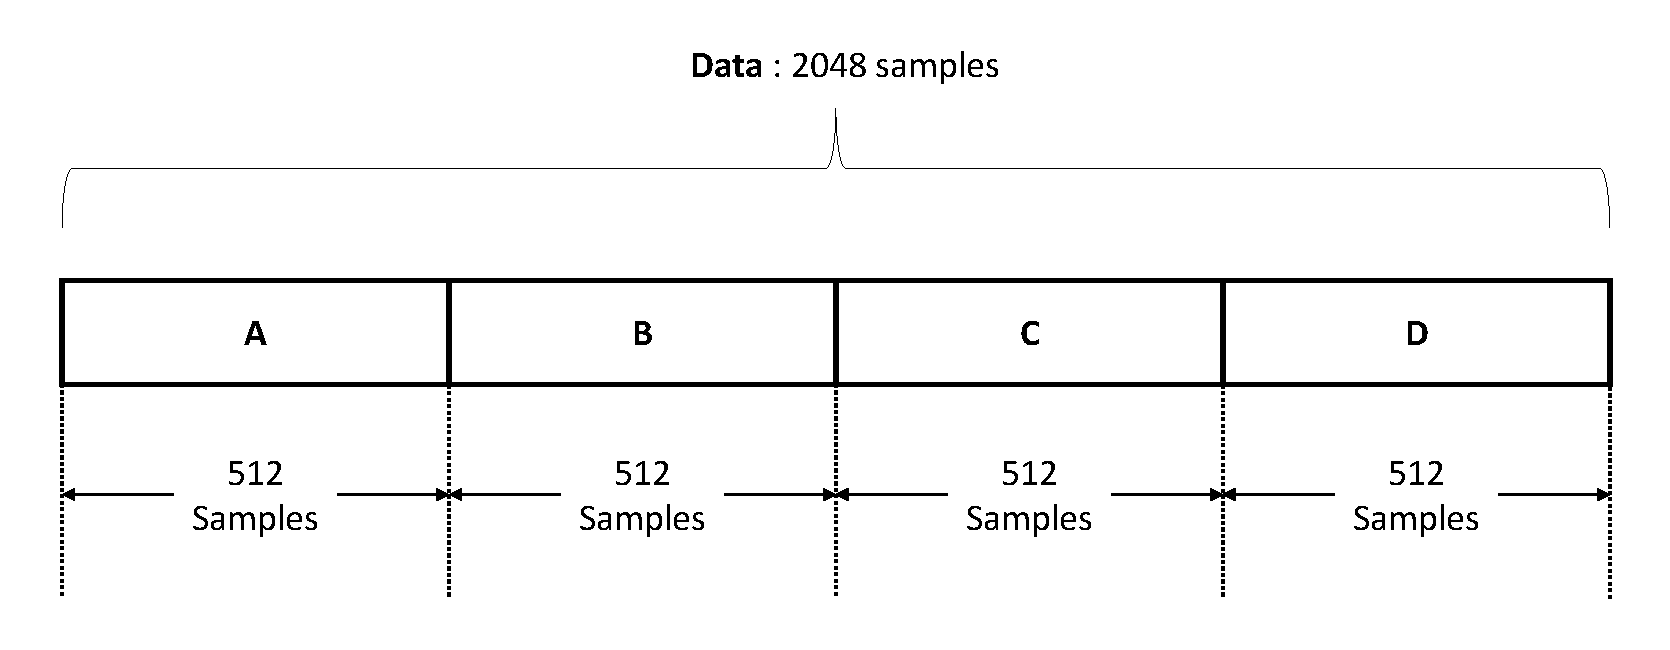
\includegraphics[width=14cm]{./algorithms/hilbert/figures/data.pdf}
	\caption{Logical flow}
	\label{data}
\end{figure}
The filtering process will start only after acquiring first two blocks $A$ and $B$ (see iteration 1 in Figure \ref{Logical flow}), which introduces delay in the system. In the iteration 1, $x(n)$ consists of 512 front Zeros, block $A$ and block $B$ which makes the total length of the $x(n)$ is $512$ x $3 = 1536$ symbols. After applying filter to the $x(n)$, we will capture the data which corresponds to the block $A$ only and discard the remaining data from each side of the filtered output.\\
\begin{figure}[h]
	\centering
	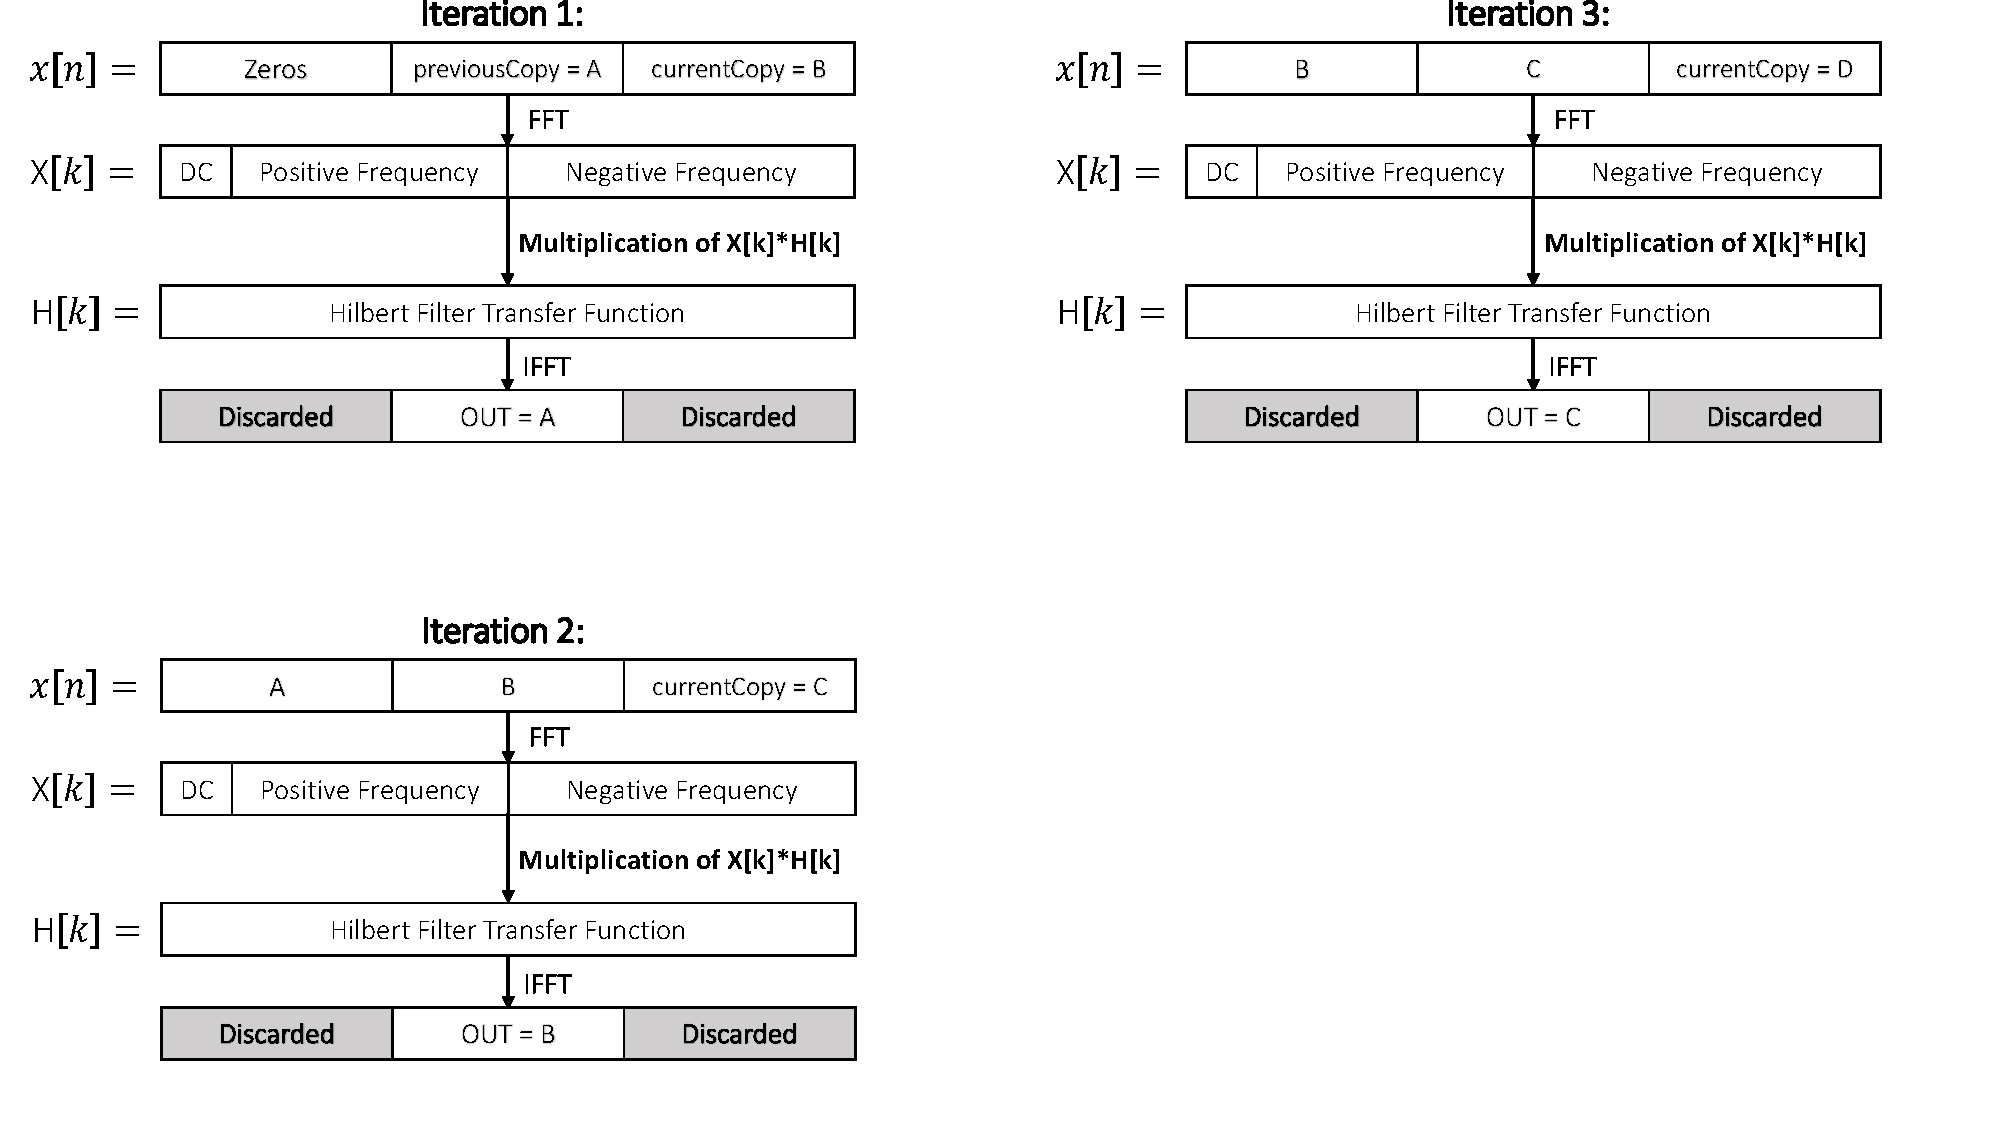
\includegraphics[width=14cm]{./algorithms/hilbert/figures/proposedLogic.pdf}
	\caption{Logical flow of real-time Hilbert transform}
	\label{Logical flow}
\end{figure}
In the next iteration 2, we'll use \textbf{previousCopy} $A$ and $B$ along with the \textbf{currentCopy} "C" and process the signal same as we did in iteration  and we will continue the procedure until the end of the sequence.
\subsection*{Real-time Hilbert transform : Test setup}
\begin{figure}[h]
	\centering
	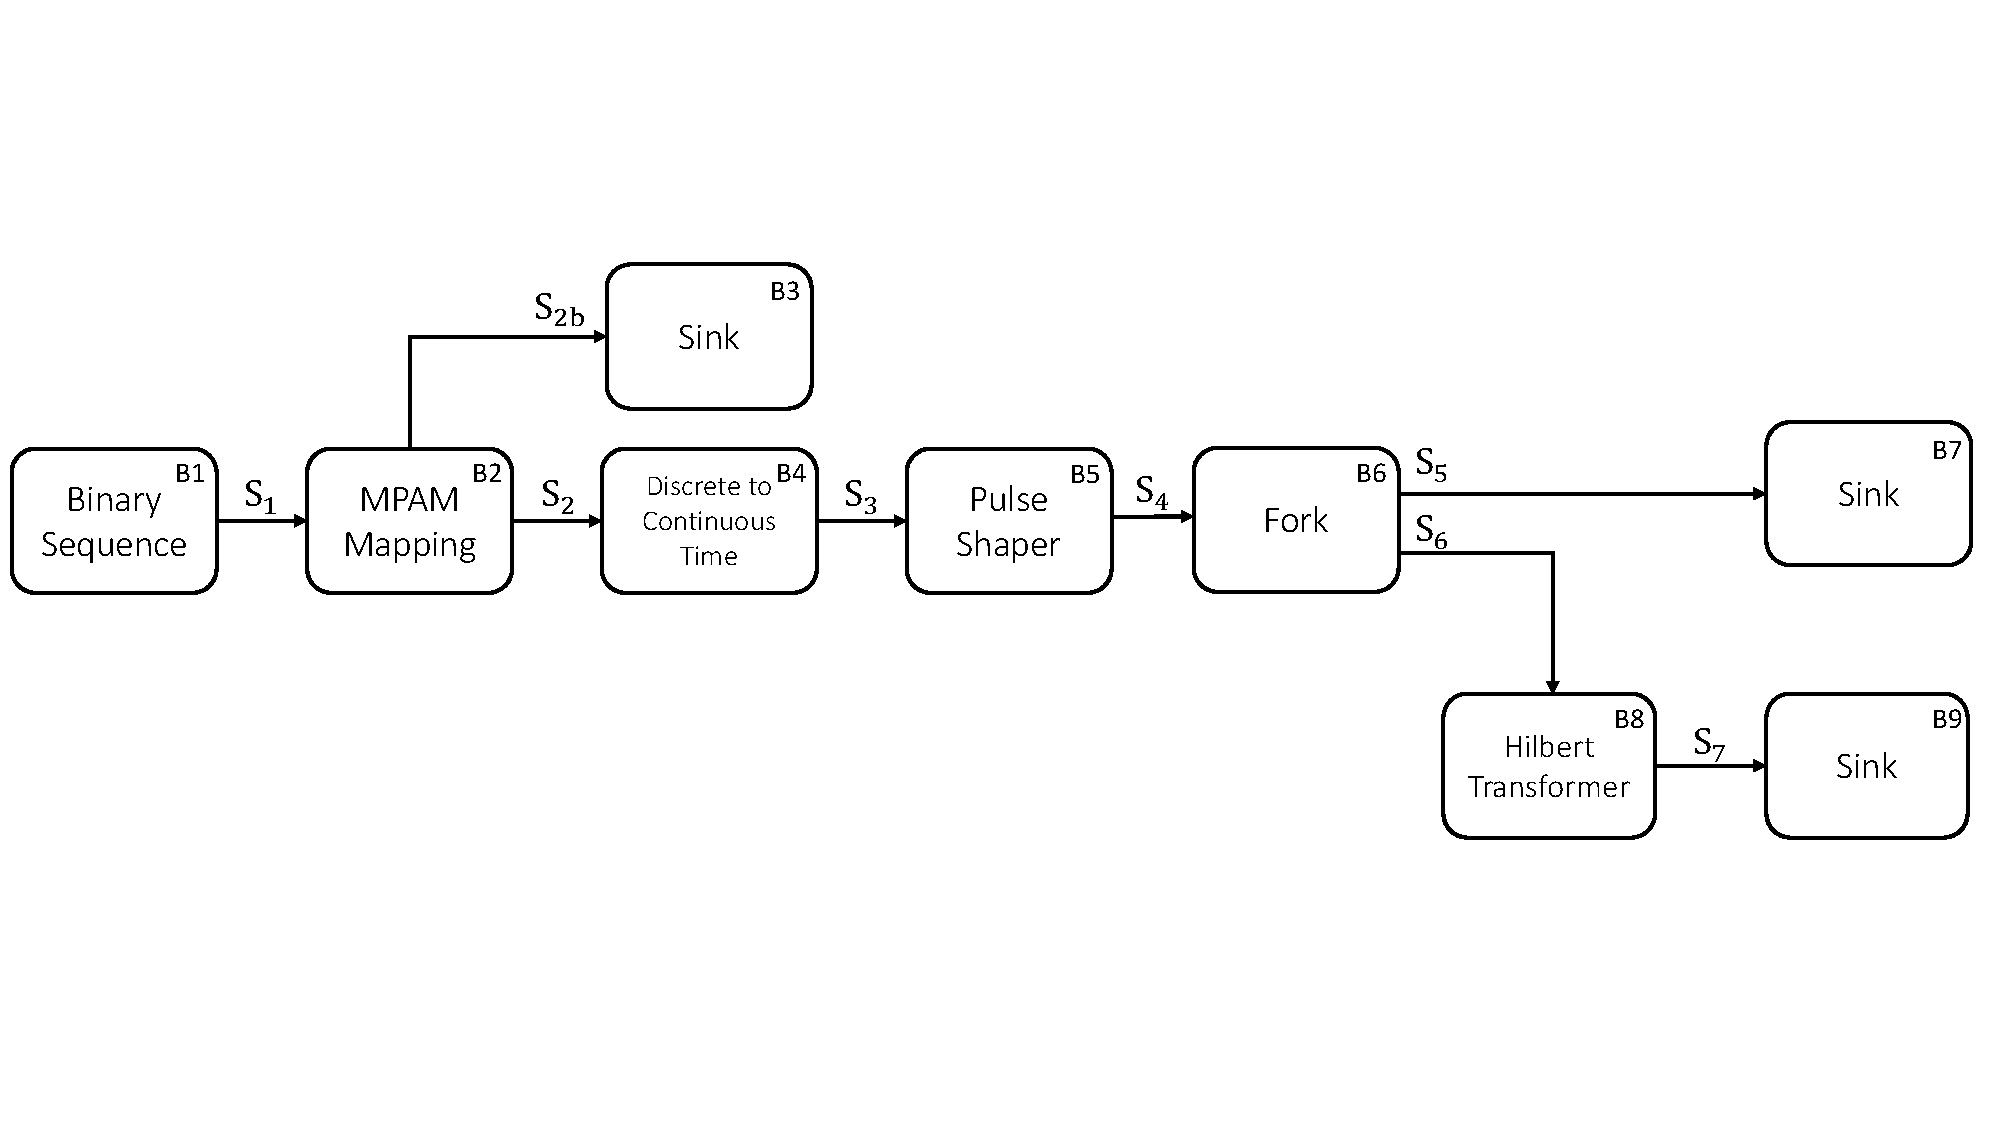
\includegraphics[width=14cm]{./algorithms/hilbert/figures/test_setup.pdf}
	\caption{Test setup for the real time Hilbert transform }\label{test_setup}
\end{figure}
\subsection*{Real-time Hilbert transform : Results}
\begin{figure}[h]
	\centering
	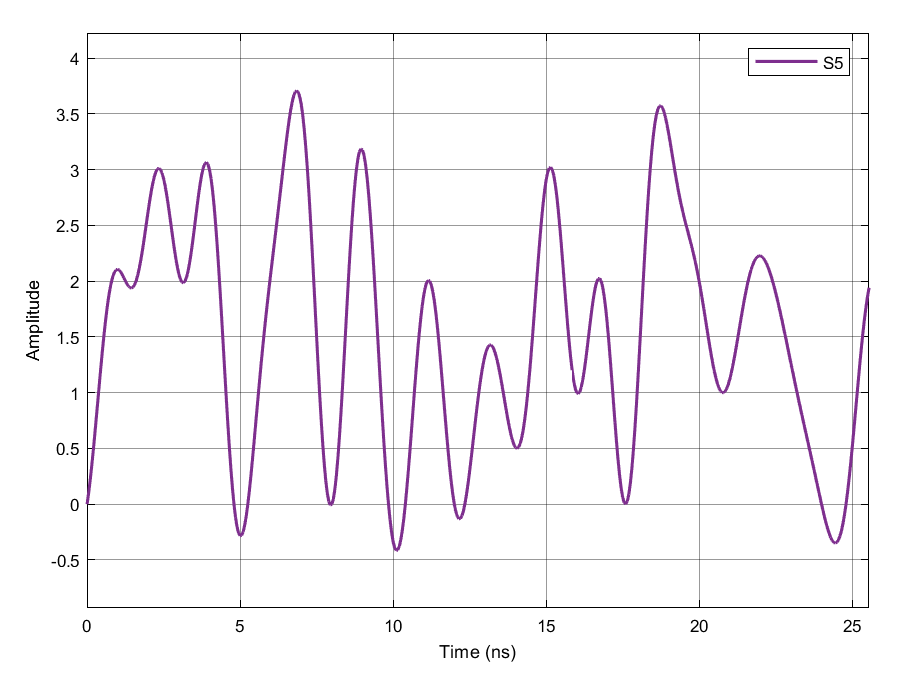
\includegraphics[width=13cm]{./algorithms/hilbert/figures/S5.eps}
	\caption{$S5$ signal}\label{S5}
\end{figure}
\begin{figure}[h]
	\centering
	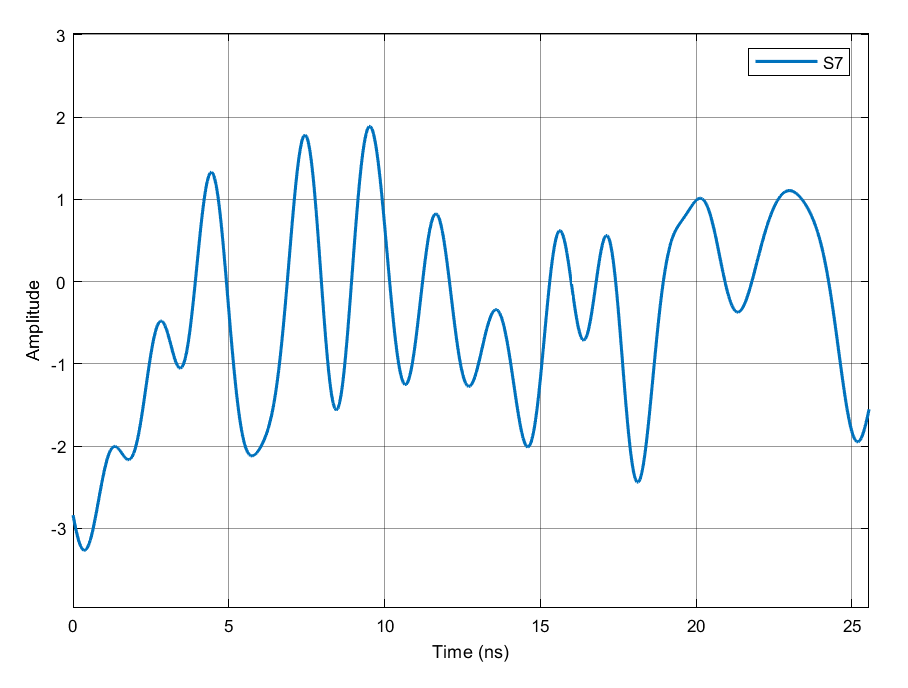
\includegraphics[width=13cm]{./algorithms/hilbert/figures/S7.eps}
	\caption{$S7$ signal}\label{S7}
\end{figure}
\textbf{Remark :} Here, we have used method 2 to generate analytical signal using Hilbert transform. If you want to use method 1 then you should use $ifft$ in place of $fft$ and vice-versa.



% bibliographic references for the section ----------------------------
\clearpage
\printbibliography[heading=subbibliography]
\end{refsection}
\addcontentsline{toc}{subsection}{Bibliography}
\cleardoublepage
% --------------------------------------------------------------------- 

